%卒論概要テンプレート ver. 4.0

\documentclass[uplatex,twocolumn,dvipdfmx]{jsarticle}
\usepackage[top=22mm,bottom=22mm,left=22mm,right=22mm]{geometry}
\setlength{\columnsep}{11mm}
\usepackage[T1]{fontenc}
\usepackage{txfonts}
\usepackage[expert,deluxe]{otf}
\usepackage[dvipdfmx,hiresbb]{graphicx}
\usepackage[dvipdfmx]{hyperref}
\usepackage{pxjahyper}
\usepackage{secdot}





%タイトルと学生番号,名前だけ編集すること
\title{\vspace{-5mm}\fontsize{14pt}{0pt}\selectfont 分散型SNSにおけるユーザの潜在要求分析}
\author{\normalsize プロジェクトマネジメントコース 矢吹研究室 1442037 加藤 健弥}
\date{}
\pagestyle{empty}
\begin{document}
\fontsize{10.5pt}{\baselineskip}\selectfont
\maketitle





%以下が本文
\section{序論}\label{序論}
スマートフォンなどの普及により,手軽にインターネットへの接続が可能になった.そのため,TwitterやFacebookなどの様々なSNS(ソーシャルネットワークサービス)が注目されるようになった.近年ではMastodonという新たなSNSの利用者が増えてきている.

Mastodonとは2016年に公開されたオープンソースソフトウェアであり,誰でも自由にサーバを立てて運用できる.そのため,TwitterやFacebookのような利用者が一つのサーバにログインする中央集権型のサービスに対してMastodonの利用者は管理者も設置場所も異なるサーバにあるインスタンスにログインする分散型のサービスである.

インスタンスとは,Mastodonを運用しているそれぞれのサーバのことである.そのため,利用者は別のインスタンスの利用者とはつながっていない.しかしインスタンス同士が連合という形で結びつくことができるため,別のインスタンスであっても連合であれば利用者同士でつながることができる\cite{Mastodon}.




\section{目的}

TwitterとMastodonで,投稿される話題に違いがあるかを,つぶやきを定量的に分析することによって調査する.

\section{手法}

Twitter API,Mastodon APIを使用し,Twitterと30のMastodonのインスタンスから1つのインスタンスごとに無作為に100のつぶやきを集める.その集めたつぶやきをWord2vecによってベクトル化する.その結果をTwitterとMastodonの各インスタンス同士で主成分分析する.


\section{結果}

Twitterと30のMastodonのインスタンスを対象に調査した.図\ref{mstdn}はTwitterと話題が自由なインスタンスであるmstdn.jpの100のつぶやきをベクトル化し,主成分分析をした結果である.図\ref{ika}はTwitterとスプラトゥーンの話題が中心のインスタンスであるika.queloud.netの100のつぶやきをベクトル化し,主成分分析した結果である.
\vspace{-1.0zh}
\begin{figure}[h]
\begin{tabular}{cc}
\begin{minipage}{0.5\hsize}
\begin{center}
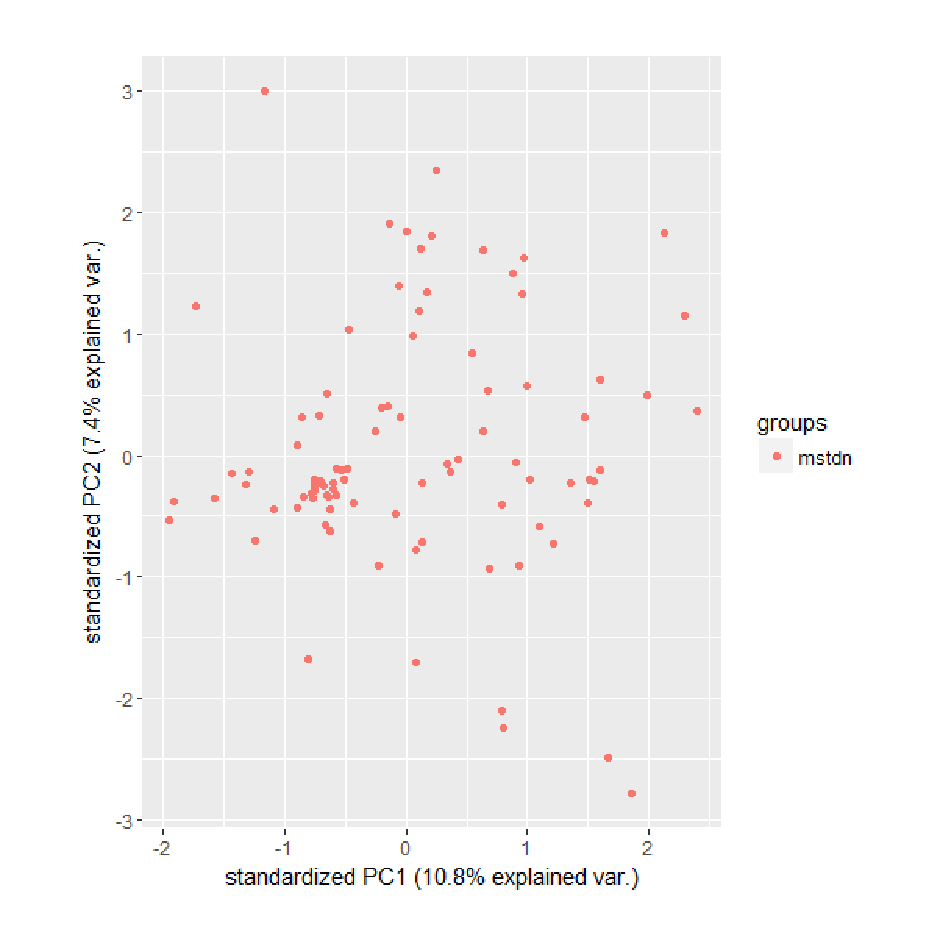
\includegraphics[width=40mm,clip]{mstdn.pdf}
\caption{話題が自由なインスタンス}
\label{mstdn}
\end{center}
\end{minipage}
\begin{minipage}{0.5\hsize}
\begin{center}
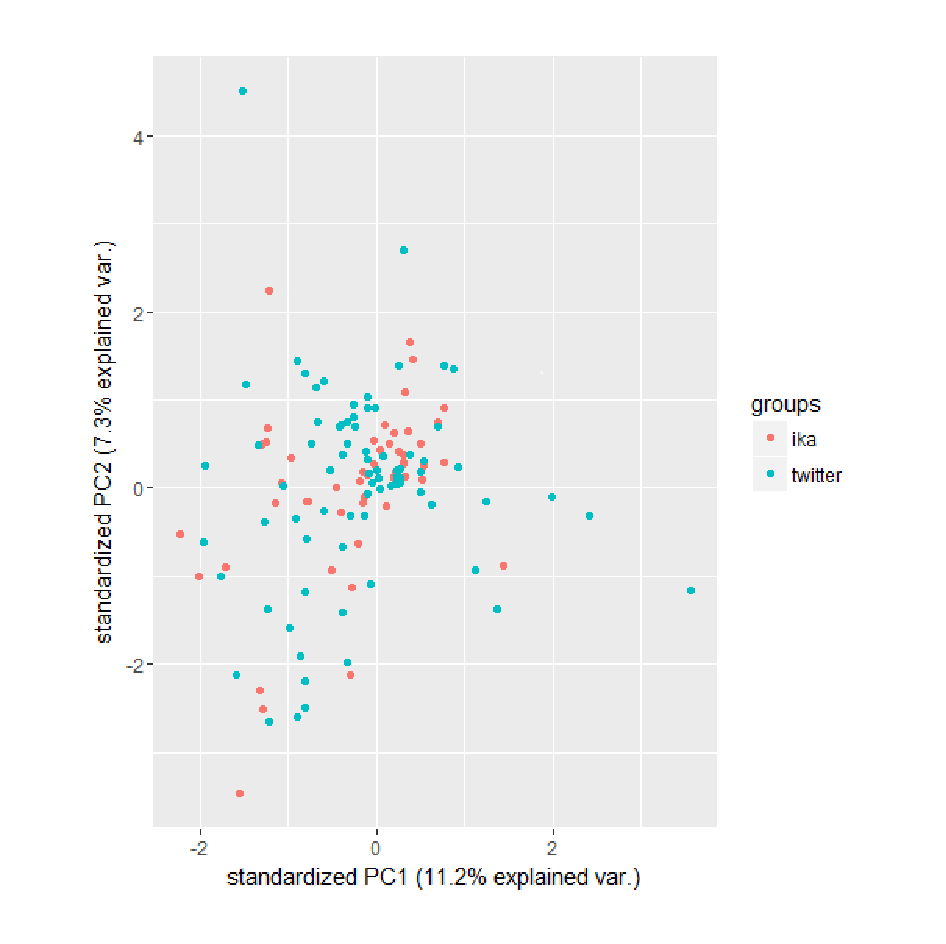
\includegraphics[width=40mm,clip]{ika.pdf}
\caption{スプラトゥーンが話題の中心のインスタンス}
\label{ika}
\end{center} 
\end{minipage}
\end{tabular}
\end{figure}
\vspace{-1.0zh}
\section{考察}

主成分分析の結果を可視化したバイプロットでは,話題が幅広いTwitterのつぶやきは拡散し,話題が限定されているMastodonのつぶやきは局所化することが予想されたのだが,分析結果は図のように,両者に明確な違いは見られなかった.このことは,Word2vecと主成分分析という方法では,人間が簡単に理解しているような,話題の違いを検出できないことを示唆している.

\section{結論}

本研究で用いたWord2vecと主成分分析という手法で話題の広さの違いを識別することは困難だということが分かった.つぶやき単体ではなく,大量のつぶやきをまとめてベクトル化する手法を試みることが今後の課題であろう.


\bibliographystyle{junsrt}
\bibliography{biblio}%「biblio.bib」というファイルが必要.

\end{document}